\documentclass{article}

\usepackage{pgfplots}
\usepackage[margin=0cm]{geometry}

\pgfplotsset{compat=1.13}
\usepgfplotslibrary{patchplots}

\begin{document}

\parskip=20pt
\parindent=0pt


\def\PLOTx[#1]{%
	\addplot[point meta=explicit,#1]
	coordinates {
	(0,0) [\pgfkeysvalueof{/CC/00}] (1,0) [\pgfkeysvalueof{/CC/10}] (2,0) [\pgfkeysvalueof{/CC/20}]

	(0,1) [\pgfkeysvalueof{/CC/01}] (1,1) [\pgfkeysvalueof{/CC/11}] (2,1) [\pgfkeysvalueof{/CC/21}]

	(0,2) [\pgfkeysvalueof{/CC/02}] (1,2) [\pgfkeysvalueof{/CC/12}] (2,2) [\pgfkeysvalueof{/CC/22}]
	};
}%

\pgfkeys{
	/CC/none/.initial=,
	/CC/00/.initial={0},
	/CC/10/.initial={1},
	/CC/20/.initial={2},
	%
	/CC/01/.initial={3},
	/CC/11/.initial={4},
	/CC/21/.initial={5},
	%
	/CC/02/.initial={6},
	/CC/12/.initial={7},
	/CC/22/.initial={8},
	%
}

\foreach \A/\spacing in {%
11/~,%
	none/\\,%
	00/~,10/~,20/\\,%
	01/~,11/~,21/\\,%
	02/~,12/~,22/\\%
}{%
	\message{generating \A...^^J}%
	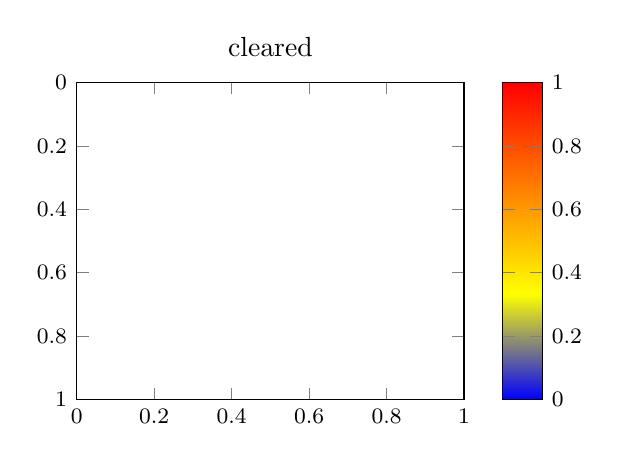
\begin{tikzpicture}
	%\tracingmacros=2 \tracingcommands=2
		\begin{axis}[
			small,
			colorbar,
			colorbar style={lua backend/.try=false},
			axis on top,
			y dir=reverse,
			%enlargelimits={abs=1},
			enlargelimits=false,
			shader=interp,
			title=\A\space cleared,
		]

		\PLOTx[surf, /CC/\A={nan}]

		\PLOTx[mark=*,scatter,
			mark size=4pt,only marks]
			
		\end{axis}
	\end{tikzpicture}\spacing
}
\end{document}

